\documentclass[12pt,a4paper]{article}

% ── Packages ──────────────────────────────────────────────────────────
\usepackage[french]{babel}
\usepackage[T1]{fontenc}
\usepackage[utf8]{inputenc}
\usepackage{geometry}
\geometry{margin=2.5cm}
\usepackage{xcolor}
\usepackage{listings}
\usepackage{graphicx}
\usepackage{hyperref}
\usepackage{titlesec}
\usepackage{fancyhdr}
\usepackage{float}
\usepackage{caption}
\usepackage{enumitem}
\usepackage{times}
\usepackage{booktabs}
\usepackage{array}
\usepackage{tikz}
\usetikzlibrary{positioning, arrows.meta, shapes.geometric, fit, backgrounds, shadows}

% ── Page style ────────────────────────────────────────────────────────
\pagestyle{fancy}
\fancyhf{}
\fancyhead[L]{\footnotesize\textit{Météo App — Rapport de projet Angular}}
\fancyhead[R]{\footnotesize\textbf{\thepage}}
\renewcommand{\headrulewidth}{0.4pt}

% ── Code listings style ──────────────────────────────────────────────
\definecolor{codebg}{RGB}{248,250,252}
\definecolor{codeframe}{RGB}{226,232,240}
\definecolor{codegreen}{RGB}{22,163,74}
\definecolor{codeblue}{RGB}{37,99,235}
\definecolor{codegray}{RGB}{100,116,139}
\definecolor{codepurple}{RGB}{147,51,234}

\lstdefinestyle{angular}{
    language          = Java,
    backgroundcolor   = \color{codebg},
    basicstyle        = \ttfamily\small,
    breakatwhitespace = false,
    breaklines        = true,
    captionpos        = b,
    commentstyle      = \color{codegray}\itshape,
    extendedchars     = true,
    frame             = single,
    rulecolor         = \color{codeframe},
    keywordstyle      = \color{codepurple}\bfseries,
    numbers           = left,
    numberstyle       = \tiny\color{codegray},
    tabsize           = 2,
    stringstyle       = \color{codegreen},
    showstringspaces  = false,
    literate          = {°}{{\textdegree}}1
                           {é}{{\'e}}1
                           {è}{{\`e}}1
                           {ê}{{\^e}}1
                           {à}{{\`a}}1
                           {â}{{\^a}}1
                           {ù}{{\`u}}1
                           {ç}{{\c{c}}}1
                           {î}{{\^i}}1
                           {ô}{{\^o}}1
                           {ë}{{\"e}}1
                           {û}{{\^u}}1,
}

\lstdefinestyle{bash}{
    language          = bash,
    backgroundcolor   = \color{codebg},
    basicstyle        = \ttfamily\small,
    frame             = single,
    rulecolor         = \color{codeframe},
    numbers           = none,
}

% ── Sections formatting ───────────────────────────────────────────────
\titleformat{\section}{\Large\bfseries\color{blue!60!black}}{}{0pt}{}
\titleformat{\subsection}{\large\bfseries\color{blue!40!black}}{}{0pt}{}
\titleformat{\subsubsection}{\normalsize\bfseries}{}{0pt}{}

% ── Title page ────────────────────────────────────────────────────────
\begin{document}

\begin{titlepage}
\begin{center}
\vspace*{2cm}

{\large \textbf{Université Hassan II}}\\[0.5cm]
{\large Faculté des sciences et techniques de Mohammedia}\\[0.5cm]
{\large Filière ILISI}\\[2cm]

{\Huge \textbf{Météo App}}\\[0.3cm]
{\Large \textbf{Application de Visualisation}}\\[0.1cm]
{\Large \textbf{et de Prévisions Météorologiques}}\\[1cm]

{\large Rapport de projet}\\[0.2cm]
{\large Module : Développement Full Stack Moderne}\\[0.2cm]
{\large Encadré par : Pr. Chakri Sanae}\\[2cm]

\vfill

\begin{minipage}[t]{0.45\textwidth}
\centering
\textbf{Réalisé par :}\\[0.3cm]
Bichri Yasser\\[0.1cm]
Jounaid Ayoub
\end{minipage}
\hfill
\begin{minipage}[t]{0.45\textwidth}
\centering
\textbf{Année universitaire :}\\[0.3cm]
2025 / 2026
\end{minipage}

\vspace{1.5cm}

\end{center}
\end{titlepage}

\newpage
\section*{Resume}
\addcontentsline{toc}{section}{Resume}


\begin{center}
\fbox{\parbox{0.85\textwidth}{\centering
\vspace{0.3cm}
Météo App est une application Angular 21 complète qui illustre la mise en œuvre des composants standalone, des Signals pour la gestion d'état réactive, des formulaires réactifs, du routage paramétré, du rendu SSR, et de l'intégration d'API REST. L'application offre une expérience utilisateur riche avec des visualisations SVG animées, une recherche de villes réactive, et une comparaison de données météorologiques en temps réel.
\vspace{0.3cm}
}}
\end{center}

\vfill

\begin{center}
\textbf{Mots-clés :} Angular 21, Signals, TypeScript, Tailwind CSS, SSR, Open-Meteo, SVG, Application meteo, Composants standalone.
\end{center}

\newpage

\tableofcontents
\newpage

% ──────────────────────────────────────────────────────────────────────
\section{Introduction}
\label{sec:intro}

\subsection{Présentation du projet}

Météo App est une application web de visualisation météorologique développée avec Angular 21 dans le cadre du module \og{}Developpement Full Stack Moderne\fg{}. Elle permet à l'utilisateur de consulter les conditions météorologiques actuelles, les prévisions horaires sur 24~h, les tendances sur cinq jours avec un graphique dynamique, la qualité de l'air, et de comparer les données de deux villes côte-à-côte.

L'application exploite les API publiques d'Open-Meteo pour les données météorologiques et de géocodage, ainsi que Nominatim (OpenStreetMap) pour le géocodage inverse. Le c\oe ur du projet réside dans l'architecture Angular : composants standalone, gestion d'état réactive avec les Signals, formulaires réactifs, routage paramétré, et rendu côté serveur.

\subsection{Technologies utilisées}

\begin{itemize}[nosep]
    \item \textbf{Framework} : Angular 21 (standalone API, plus de NgModules)
    \item \textbf{Langage} : TypeScript 5.9
    \item \textbf{Gestion d'état} : Angular Signals (\texttt{signal()}, \texttt{computed()})
    \item \textbf{HTTP} : \texttt{HttpClient} d'Angular avec RxJS
    \item \textbf{Routage} : \texttt{Router} Angular (routes standalone)
    \item \textbf{Formulaires} : \texttt{ReactiveFormsModule} (\texttt{FormControl})
    \item \textbf{Styles} : Tailwind CSS v4
    \item \textbf{SSR} : Angular SSR avec serveur Express
    \item \textbf{Tests} : Vitest + \texttt{HttpTestingController}
    \item \textbf{Icones} : Angular Material Icons
    \item \textbf{API externes} : Open-Meteo, Nominatim
\end{itemize}

\subsection{Fonctionnalités de l'application}

\begin{itemize}[nosep]
    \item Recherche de villes avec autocomplétion et debounce
    \item Affichage des conditions météorologiques actuelles (température, humidité, vent)
    \item Prévisions horaires sur 24~h avec défilement horizontal
    \item Graphique SVG animé des températures sur 5~jours
    \item Indice de qualité de l'air (AQI) avec code couleur
    \item Comparaison de deux villes avec tableau et cartes jour par jour
    \item Gestion des favoris avec persistance locale
    \item Historique des dernières recherches
    \item Géolocalisation automatique
    \item Bascule entre Celsius et Fahrenheit
    \item Mode sombre
    \item Résumé textuel des conditions météorologiques
\end{itemize}

% ──────────────────────────────────────────────────────────────────────
\newpage
\section{Architecture de l'application}
\label{sec:archi}

\subsection{Structure du projet}

L'application suit la structure standard d'un projet Angular avec des composants \emph{standalone}. Tous les fichiers sources se trouvent dans le dossier \texttt{src/app/}.

\begin{lstlisting}[style=bash, caption={Arborescence du projet}]
src/
  app/
    app.ts                  # Composant racine
    app.config.ts           # Configuration globale
    app.routes.ts           # Definition des routes
    app.routes.server.ts    # Modes de rendu SSR
    weather.ts              # Service metier et interfaces
    dashboard.ts            # Composant tableau de bord
    forecast.ts             # Composant previsions 5 jours
    compare.ts              # Composant comparaison
    *.spec.ts               # Tests unitaires
  styles.css                # Configuration Tailwind
  server.ts                 # Serveur Express SSR
\end{lstlisting}

\subsection{Routage}

Les routes sont definies avec l'API standalone d'Angular :

\begin{lstlisting}[style=angular, caption={Definition des routes}]
export const routes: Routes = [
  { path: '',                        component: Dashboard },
  { path: 'forecast/:lat/:lon/:name',component: Forecast },
  { path: 'compare',                 component: Compare },
  { path: '**', redirectTo: '' },
];
\end{lstlisting}

Le routeur distingue trois vues principales :
\begin{itemize}[nosep]
    \item \textbf{Tableau de bord} (\texttt{/}) — page d'accueil avec la meteo actuelle, les prévisions horaires et la qualité de l'air
    \item \textbf{Previsions detaillees} (\texttt{/forecast/:lat/:lon/:name}) — graphique SVG et cartes sur 5~jours, accessible depuis le bouton \og{}Voir les previsions\fg{} du tableau de bord
    \item \textbf{Comparaison} (\texttt{/compare}) — comparaison de deux villes avec presets
\end{itemize}

La route \texttt{forecast} utilise \texttt{ActivatedRoute.paramMap} pour extraire les paramètres dynamiques (latitude, longitude, nom). Elle est configuree en mode \texttt{RenderMode.Server} pour le SSR afin que les coordonnees dynamiques soient correctement rendues.

\subsection{Composants et service partage}

Tous les composants partagent un unique service \texttt{WeatherManager}, injecte via \texttt{providedIn: 'root'}, garantissant un etat coherent dans toute l'application.

\begin{center}
\fbox{\parbox{0.85\textwidth}{
\textbf{Flux de donnees :}
\begin{enumerate}[nosep]
    \item L'utilisateur interagit avec un composant (clic, saisie)
    \item Le composant appelle une methode du \texttt{WeatherManager}
    \item Le service effectue une requete HTTP vers une API externe
    \item Les donnees recues mettent a jour un \texttt{signal()}
    \item Angular detecte le changement via sa détection de changements \texttt{OnPush} et re-rend la vue
\end{enumerate}
}}
\end{center}

\subsubsection{Diagramme d'architecture}

La figure~\ref{fig:architecture} illustre l'architecture globale de l'application, montrant les trois couches principales : les composants Angular, le service central, et les API externes.

\begin{figure}[H]
\centering
\begin{tikzpicture}[
    node distance = 1.2cm,
    comp/.style = {
        rectangle, rounded corners=6pt, minimum width=3.8cm, minimum height=1.6cm,
        align=center, font=\small\bfseries, text=white, drop shadow
    },
    srv/.style = {
        rectangle, rounded corners=6pt, minimum width=11cm, minimum height=1.6cm,
        align=center, font=\small\bfseries, text=white, drop shadow
    },
    apibox/.style = {
        rectangle, rounded corners=4pt, minimum width=3cm, minimum height=1.1cm,
        align=center, font=\footnotesize\bfseries, text=white, drop shadow
    },
    labelnode/.style = {
        font=\footnotesize\itshape, text=gray!70!black, align=center
    },
    arrow/.style = {
        -{Latex[length=2.5mm]}, thick, color=gray!60!black
    },
    every edge/.style = {arrow, draw}
]

% ── Layer titles ──
\node[labelnode] (l1) at (-0.5, 8.2) {Couche presentation (Angular)};
\node[labelnode] (l2) at (-0.5, 5.2) {Couche service (metier)};
\node[labelnode] (l3) at (-0.5, 1.8) {Couche API (externe)};

% ── Layer 1: Components ──
\node[comp, fill=blue!60!cyan!80] (dashboard) at (-3.8, 6.6) {Dashboard\\\footnotesize\normalfont meteo actuelle\\\footnotesize\normalfont prévisions horaires\\\footnotesize\normalfont AQI};
\node[comp, fill=blue!60!cyan!80] (forecast)   at (0, 6.6)   {Forecast\\\footnotesize\normalfont graphique SVG\\\footnotesize\normalfont cartes 5 jours};
\node[comp, fill=blue!60!cyan!80] (compare)    at (3.8, 6.6) {Compare\\\footnotesize\normalfont deux villes\\\footnotesize\normalfont tableaux/cartes};

% ── Layer 2: Service ──
\node[srv, fill=purple!70!blue!80] (service) at (0, 3.8) {WeatherManager (providedIn: 'root')\\\footnotesize\normalfont Signals : weatherData, isLoading, errorMsg, favoriteCities, ...\\\footnotesize\normalfont Methodes : configWeather, searchCities, toggleFavorite, ...};

% ── Layer 3: APIs ──
\node[apibox, fill=green!60!black!70] (meteo) at (-3.2, 0.6) {Open-Meteo\\Forecast API};
\node[apibox, fill=green!60!black!70] (aqi)   at (0, 0.6)    {Open-Meteo\\Air Quality API};
\node[apibox, fill=green!60!black!70] (geo)   at (3.2, 0.6)  {Nominatim\\Geocodage};

% ── SSR side node ──
\node[apibox, fill=orange!70!black!80] (ssr) at (7.5, 3.8) {Serveur Express\\SSR};
\node[labelnode, font=\tiny\itshape] at (7.5, 2.2) {/api/weather-briefing};

% ── Arrows: components → service ──
\draw[arrow] (dashboard.south) -- (service.north -| dashboard.south);
\draw[arrow] (forecast.south)  -- (service.north);
\draw[arrow] (compare.south)   -- (service.north -| compare.south);

% ── Arrows: service → APIs ──
\draw[arrow] (service.south west) -- ++(0,-0.3) -| (meteo.north);
\draw[arrow] (service.south)      -- ++(0,-0.7)    (aqi.north);
\draw[arrow] (service.south east) -- ++(0,-0.3) -| (geo.north);

% ── Arrows: service ↔ SSR ──
\draw[arrow] (service.east) -- ++(0.4,0) |- (ssr.west);
\draw[arrow] (ssr.west)     -- ++(-0.4,0) |- (service.east);

% ── Return arrows (API → Service) ──
\draw[arrow, dashed] (meteo.south) -- ++(0,-0.4) -- ++(4.2,0) |- (service.south);
\draw[arrow, dashed] (aqi.south)   -- ++(0,-0.4) -- ++(4.2,0) |- (service.south);
\draw[arrow, dashed] (geo.south)   -- ++(0,-0.4) -- ++(4.2,0) |- (service.south);

\end{tikzpicture}
\caption{Architecture de l'application Météo App}
\label{fig:architecture}
\end{figure}

% ──────────────────────────────────────────────────────────────────────
\newpage
\section{Le service WeatherManager et la gestion d'état}
\label{sec:service}

\subsection{Présentation du service}

Le \texttt{WeatherManager} est le c\oe ur metier de l'application. Déclaré avec \texttt{providedIn: 'root'}, il agit comme un singleton et centralise toute la logique : appels API, gestion des signaux, persistance \texttt{localStorage}, et transformations de données.

\begin{lstlisting}[style=angular, caption={Declaration et signaux du service}]
@Injectable({ providedIn: 'root' })
export class WeatherManager {
  private http = inject(HttpClient);

  // Signaux d'etat
  readonly températureUnit   = signal<'C' | 'F'>('C');
  readonly isDarkMode        = signal<boolean>(false);
  readonly currentCity       = signal<City>(defaultCity);
  readonly weatherData       = signal<WeatherData | null>(null);
  readonly isLoading         = signal<boolean>(false);
  readonly errorMsg          = signal<string | null>(null);
  readonly recentSearches    = signal<City[]>([]);
  readonly favoriteCities    = signal<City[]>([]);
  readonly compareCityA      = signal<City | null>(null);
  readonly compareCityB      = signal<City | null>(null);
  readonly compareDataA      = signal<WeatherData | null>(null);
  readonly compareDataB      = signal<WeatherData | null>(null);
  readonly isComparingLoading= signal<boolean>(false);
  readonly aiSummary         = signal<string | null>(null);
  readonly isAiLoading       = signal<boolean>(false);
}
\end{lstlisting}

\subsection{Angular Signals : une gestion d'état réactive}

L'application utilise exclusivement les \texttt{Signal}s pour la gestion d'état. Ce choix permet :

\begin{itemize}[nosep]
    \item Une \textbf{réactivité fine} : Angular détecte précisément quel signal a change et ne re-vérifie que le fragment du template concerné
    \item Une \textbf{gestion simplifiée} : pas de \texttt{BehaviorSubject}, \texttt{async pipe} ou \texttt{Subscription} à gérer pour l'état local
    \item Une \textbf{performance accrue} grace au nouveau systeme de détection de changements
    \item \textbf{Aucune désinscription manuelle} : contrairement aux abonnements RxJS, les signaux ne nécessitent pas de \texttt{ngOnDestroy}
\end{itemize}

\subsection{Diagramme de flux de donnees}

La figure~\ref{fig:dataflow} illustre le parcours complet d'une interaction utilisateur, depuis la saisie dans le champ de recherche jusqu'a la mise a jour de l'interface.

\begin{figure}[H]
\centering
\begin{tikzpicture}[
    box/.style = {
        rectangle, rounded corners=4pt, minimum width=3cm, minimum height=1cm,
        align=center, font=\small, drop shadow, text=white
    },
    arrow/.style = {
        -{Latex[length=2mm]}, thick, color=gray!50!black
    },
    label/.style = {
        font=\footnotesize\itshape, text=gray!60!black, above, midway
    }
]

% Row 1 ── User action
\node[box, fill=blue!70!cyan!80]           (user) at (-5.5, 2.5) {Utilisateur};
\node[box, fill=blue!70!cyan!80]           (comp) at (-2.2, 2.5) {Composant};
\node[box, fill=purple!70!blue!80]         (srv)  at (1.2, 2.5)  {WeatherManager};
\node[box, fill=green!60!black!70]         (api)  at (4.8, 2.5)  {API externe};

% Row 2 ── Data flow
\node[box, fill=purple!70!blue!80]         (sig)  at (1.2, -0.2) {Signal\\\footnotesize\normalfont .set() / .update()};
\node[box, fill=blue!70!cyan!80]           (view) at (4.8, -0.2) {Template\\\footnotesize\normalfont re-rendu};

% Horizontal arrows row 1
\draw[arrow] (user.east) -- node[label] {saisie}          (comp.west);
\draw[arrow] (comp.east) -- node[label] {methode}         (srv.west);
\draw[arrow] (srv.east)  -- node[label] {HTTP GET}        (api.west);

% Vertical arrow: API → Signal
\draw[arrow] (api.south) -- ++(0,-0.7) -- ++(-3.6,0)
    node[midway, above, font=\footnotesize\itshape] {reponse JSON}
    |- (sig.east);

% Horizontal arrow row 2
\draw[arrow] (sig.east)  -- node[label] {notification}    (view.west);

% Return arrow: View → User
\draw[arrow, dashed, rounded corners]
    (view.north) -- ++(0,0.6) -- ++(-7.7,0)
    node[midway, above, font=\footnotesize\itshape] {affichage}
    |- (user.north);

\end{tikzpicture}
\caption{Flux de donnees lors d'une interaction utilisateur}
\label{fig:dataflow}
\end{figure}

\subsection{Signal calculé (computed)}

Le signal dérivé \texttt{chartData} se recalcule automatiquement dès que \texttt{weatherData} change :

\begin{lstlisting}[style=angular, caption={Signal computed pour les coordonnees du graphique}]
readonly chartData = computed(() => {
  const data = this.weatherData();
  if (!data) return null;
  return this.computeChartCoordinates(data.forecast);
});
\end{lstlisting}

Ce mécanisme garantit que les coordonnées SVG du graphique sont toujours synchronisées avec les donnees sans intervention manuelle.

\subsection{Gestion des appels API parallèles}

La méthode \texttt{configWeather()} illustre le chargement parallèle de deux API via \texttt{forkJoin} :

\begin{lstlisting}[style=angular, caption={Chargement parallele des API meteo et qualité de l'air}]
configWeather(city: City): Observable<WeatherData> {
  const params = `latitude=${city.latitude}
                  &longitude=${city.longitude}`;

  const weather$ = this.http.get<OpenMeteoResponse>(
    `https://api.open-meteo.com/v1/forecast?${params}
     &current=température_2m,relative_humidity_2m,...`
  );

  const aqi$ = this.http.get<AqiApiResponse>(
    `https://air-quality-api.open-meteo.com/v1/air-quality?${params}
     &current=european_aqi,us_aqi,pm2_5,pm10,ozone`
  ).pipe(catchError(() => of(null)));

  return forkJoin({ weather: weather$, aqi: aqi$ }).pipe(
    map(({ weather, aqi }) => this.mapToWeatherData(weather, aqi, city))
  );
}
\end{lstlisting}

Le \texttt{catchError(() => of(null))} sur l'API AQI est un choix délibéré : si la qualité de l'air est indisponible, l'application continue de fonctionner et affiche simplement les données météorologiques.

% ──────────────────────────────────────────────────────────────────────
\newpage
\section{Fonctionnalités détaillées}
\label{sec:features}

\subsection{Recherche de villes avec autocomplétion}

\subsubsection{Mecanisme}

La recherche de villes est implémentée dans le composant \texttt{Dashboard} via un \texttt{FormControl} reactif. Le mecanisme repose sur une combinaison d'opérateurs RxJS :

\begin{lstlisting}[style=angular, caption={Autocompletion avec debounce et switchMap}]
ngOnInit() {
  this.sub = this.searchCtrl.valueChanges.pipe(
    debounceTime(350),              // Attend 350ms apres la derniere frappe
    distinctUntilChanged(),         // Ignore les valeurs identiques
    switchMap(value => {
      if (!value || value.trim().length < 2) {
        return of([]);              // Pas de requete avant 2 caracteres
      }
      this.isSuggesting.set(true);
      return this.manager.searchCities(value);
    })
  ).subscribe(cities => {
    this.suggestions.set(cities);
    this.isSuggesting.set(false);
  });
}
\end{lstlisting}

\subsubsection{Le rôle du switchMap}

L'opérateur \texttt{switchMap} est essentiel : si l'utilisateur continue de taper avant que la requete ne revienne, il annule automatiquement la requête précédente et en émet une nouvelle. Cela evite :
\begin{itemize}[nosep]
    \item Les appels API superflus
    \item Les \emph{race conditions} (affichage de suggestions pour une ancienne requête)
    \item La congestion réseau
\end{itemize}

\subsubsection{Appel API}

La méthode \texttt{searchCities()} interroge l'API de géocodage d'Open-Meteo :

\begin{lstlisting}[style=angular, caption={Requete de géocodage}]
searchCities(query: string): Observable<City[]> {
  return this.http.get<SearchResultItem>(
    `https://geocoding-api.open-meteo.com/v1/search
     ?name=${query}&count=10&language=en&format=json`
  ).pipe(
    map(response => response.results?.map(item => ({
      id: item.id,
      name: item.name,
      latitude: item.latitude,
      longitude: item.longitude,
      country: item.country ?? '',
      country_code: item.country_code,
      admin1: item.admin1,
    })) ?? [])
  );
}
\end{lstlisting}

Les résultats sont affichés dans un panneau déroulant positionné en absolu sous le champ de saisie. Chaque suggestion est cliquable et déclénche \texttt{selectCity()} :

\begin{lstlisting}[style=angular, caption={Selection d'une ville suggeree}]
selectSuggestedCity(city: City) {
  this.manager.selectCity(city);
  this.suggestions.set([]);    // Vide les suggestions
  this.searchCtrl.setValue('', { emitEvent: false });
}
\end{lstlisting}

Ce meme mécanisme est dupliqué dans le composant \texttt{Compare} pour les deux champs de recherche (Ville A et Ville B) de manière indépendante.

\newpage
\subsection{Prévisions horaires (Hourly Forecast)}

\subsubsection{Récupération des données}

Les prévisions horaires sont incluses dans la requête principale a l'API Open-Meteo Forecast. Le paramètre \texttt{hourly} demande les données heure par heure :

\begin{lstlisting}[style=angular, caption={Parametres de la requete horaire}]
&hourly=température_2m,
       precipitation_probability,
       weather_code,
       wind_speed_10m
\end{lstlisting}

L'API retourne 24~valeurs (une par heure) pour chaque champ, stockées dans \texttt{data.hourly} sous forme de tableau \texttt{HourlyForecast[]}.

\subsubsection{Affichage dans le template}

Le template utilise une bouclé \texttt{@for} avec défilement horizontal :

\begin{lstlisting}[style=angular, caption={Template du bloc des prévisions horaires}]
@if (data.hourly.length > 0) {
  <div class="p-6 md:p-8 bg-white border-b border-slate-100">
    <h3>Hourly Forecast</h3>
    <div class="flex gap-3 overflow-x-auto pb-2 scrollbar-thin">
      @for (hour of data.hourly; track hour.time) {
        @let hCond = getCond(hour.weatherCode);
        <div class="flex flex-col items-center gap-1.5
                    min-w-[64px] p-3 bg-slate-50 rounded-xl
                    border border-slate-100 shrink-0">
          <span>{{ manager.formatHour(hour.time) }}</span>
          <span class="material-icons {{ hCond.textColor }}">
            {{ hCond.icon }}
          </span>
          <span>{{ formatTemp(hour.température, ...) }}</span>
          @if (hour.precipitationProbability > 0) {
            <span>{{ hour.precipitationProbability }}%</span>
          }
        </div>
      }
    </div>
  </div>
}
\end{lstlisting}

\subsubsection{Détails d'implémentation}

Plusieurs aspects techniques sont a noter :

\begin{itemize}[nosep]
    \item \textbf{Défilement horizontal} : la classe \texttt{overflow-x-auto} permet le scroll, et \texttt{scrollbar-thin} est un style personnalisé défini dans \texttt{styles.css}
    \item \textbf{\texttt{shrink-0}} : chaque carte horaire conserve sa largeur minimale (\texttt{min-w-[64px]}) sans etre compressée
    \item \textbf{Icones dynamiques} : la fonction \texttt{getCond()} traduit le code meteorologique WMO en icône Material et couleur via l'objet \texttt{WeatherCondition}
    \item \textbf{Probabilité de précipitation} : affichée uniquement si supérieure à 0\%, pour ne pas surcharger l'interface
\end{itemize}

\subsection{Graphique des températures sur 5~jours}

\subsubsection{Principe general}

Le composant \texttt{Forecast} genere un graphique SVG inline montrant l'evolution des températures maximales (rouge) et minimales (bleu) sur 5~jours. Ce graphique est entierement calcule et dessine en TypeScript, sans bibliotheque de charting externe.

\subsubsection{Calcul des coordonnees}

La méthode \texttt{computeChartCoordinates()} transforme les donnees numeriques en coordonnees pixels :

\begin{lstlisting}[style=angular, caption={Calcul des coordonnees SVG}]
private computeChartCoordinates(list: DailyForecast[]) {
  const width = 600, height = 240;
  const paddingX = 50, paddingY = 40;
  const count = list.length;
  const xSpace = (width - paddingX * 2) / (count - 1);

  const globalMax = Math.max(...list.map(d => d.tempMax));
  const globalMin = Math.min(...list.map(d => d.tempMin));
  let span = globalMax - globalMin;
  if (span === 0) span = 1;

  const pointsMax = list.map((d, i) => {
    const x = paddingX + i * xSpace;
    const y = height - paddingY -
      ((d.tempMax - globalMin) / span) * (height - paddingY * 2);
    return { x, y, val: d.tempMax, label: dayNames[...] };
  });

  const lineMax = pointsMax.reduce(
    (p, pt, i) => i === 0
      ? `M ${pt.x} ${pt.y}`
      : `${p} L ${pt.x} ${pt.y}`, ''
  );

  return { pointsMax, pointsMin, lineMax, lineMin,
           pathMaxArea, pathMinArea };
}
\end{lstlisting}

\subsubsection{Structure du SVG}

Le SVG est construit avec les elements suivants :
\begin{itemize}[nosep]
    \item \textbf{Grille} : lignes horizontales en pointilles (\texttt{stroke-dasharray}) pour les reperes de température
    \item \textbf{Lignes de température} : chemins \texttt{<path>} rouges (max) et bleus (min) avec une epaisseur de 3px
    \item \textbf{Aires remplies} : zones sous les courbes avec un degrade (\texttt{<linearGradient>}) rose et bleu
    \item \textbf{Points de donnees} : cerclés \texttt{<circlé>} blancs avec bordure coloree
    \item \textbf{Etiquettes} : textes \texttt{<text>} pour les valeurs et les noms de jours
\end{itemize}

\subsubsection{Animation du trace}

L'animation utilise la technique du \texttt{stroke-dasharray} / \texttt{stroke-dashoffset} :

\begin{lstlisting}[style=angular, caption={Animation SVG avec stroke-dasharray}]
animateChart() {
  const svg = this.chartData();
  if (!svg) return;
  const length = Math.max(svg.lineMax.length * 3, 2000);
  this.chartDasharray = String(length);
  this.chartDashoffset = String(length);

  requestAnimationFrame(() => {
    this.chartDashoffset = '0';  // Declénche l'animation
  });
}
\end{lstlisting}

Le principe est le suivant :
\begin{enumerate}[nosep]
    \item Le chemin est initialement masque avec \texttt{stroke-dashoffset} egal a la longueur totale
    \item \texttt{requestAnimationFrame} modifie la valeur a 0
    \item Le navigateur interpole et le chemin \og{}se dessine\fg{} progressivement
    \item Une fois terminee, les cerclés des points apparaissent avec une animation d'echelle
\end{enumerate}

\newpage
\subsection{Comparaison de deux villes}

\subsubsection{Architecture}

Le composant \texttt{Compare} gere deux formulaires de recherche independants (Ville A et Ville B) et un ensemble de boutons de presets. Lorsque les deux villes sont selectionnees, les donnees sont chargees en parallele via \texttt{forkJoin} :

\begin{lstlisting}[style=angular, caption={Chargement parallele pour la comparaison}]
fetchComparisonDetails() {
  this.isComparingLoading.set(true);

  forkJoin({
    dataA: this.configWeather(this.compareCityA()!),
    dataB: this.configWeather(this.compareCityB()!),
  }).subscribe({
    next: ({ dataA, dataB }) => {
      this.compareDataA.set(dataA);
      this.compareDataB.set(dataB);
      this.isComparingLoading.set(false);
    },
    error: () => this.isComparingLoading.set(false),
  });
}
\end{lstlisting}

\subsubsection{Boutons de presets}

Des boutons de presets permettent de charger rapidement des paires de villes celebrees :

\begin{lstlisting}[style=angular, caption={Preset de comparaison}]
applyPreset('London', 51.5085, -0.1257, 'United Kingdom',
            'New York', 40.7143, -74.006, 'United States')
\end{lstlisting}

Chaque preset definit les deux villes avec leurs coordonnees exactes et déclénche \texttt{fetchComparisonDetails()}.

\subsubsection{Affichage des resultats}

Les donnees sont presentees sous deux formes :

\begin{enumerate}[nosep]
    \item \textbf{Bandeau d'intelligence comparative} : affiche la difference de température entre les deux villes avec un message dynamique (\og{}plus chaud\fg{}, \og{}plus froid\fg{}, \og{}identique\fg{})
    \item \textbf{Tableau de comparaison} : un tableau HTML semantique (\texttt{<table>}) avec les colonnes \og{}Element atmospherique\fg{}, \og{}Ville A\fg{}, \og{}Ville B\fg{} et les lignes : Temperature, Ressenti, Condition, Humidite, Vent
    \item \textbf{Cartes journalieres} : pour chaque jour, les températures max/min des deux villes sont affichees cote-a-cote avec un indicateur de difference
\end{enumerate}

\newpage
\subsection{Qualite de l'air (AQI)}

\subsubsection{Donnees}

L'indice de qualité de l'air est recuperee via l'API Open-Meteo Air Quality. Cinq indicateurs sont affiches :

\begin{lstlisting}[style=angular, caption={Parametres AQI}]
&current=european_aqi,us_aqi,pm2_5,pm10,ozone
\end{lstlisting}

\subsubsection{Code couleur}

La fonction \texttt{getAQIInfo()} attribue une couleur et un libelle a chaque valeur :

\begin{lstlisting}[style=angular, caption={Fonction de code couleur AQI}]
export function getAQIInfo(aqi: number | null) {
  if (aqi === null) return { label: 'N/A', color: 'text-slate-400' };
  if (aqi <= 20)  return { label: 'Good',       color: 'text-green-500' };
  if (aqi <= 40)  return { label: 'Fair',       color: 'text-lime-500' };
  if (aqi <= 60)  return { label: 'Moderate',   color: 'text-yellow-500' };
  if (aqi <= 80)  return { label: 'Poor',       color: 'text-orange-500' };
  return                { label: 'Very Poor',   color: 'text-red-500' };
}
\end{lstlisting}

\subsubsection{Affichage}

Les donnees sont presentees dans une grille de 5 colonnes avec des cartes individuelles :

\begin{lstlisting}[style=angular, caption={Template de la grille AQI}]
<div class="grid grid-cols-2 md:grid-cols-5 gap-3">
  @for (item of aqiItems; track item.label) {
    <div class="bg-slate-50 rounded-xl p-3 border
                border-slate-100 text-center">
      <span class="text-[9px] text-slate-400 uppercase font-bold">
        {{ item.name }}
      </span>
      <span class="text-lg font-bold {{ item.color }}">
        {{ item.value }}
      </span>
      <span class="text-[9px] text-slate-500 font-medium">
        {{ item.unit }}
      </span>
    </div>
  }
</div>
\end{lstlisting}

\subsection{Favoris et villes recentes}

\subsubsection{Gestion des favoris}

Les favoris sont stockes dans \texttt{localStorage} sous la clé \texttt{meteo\_favorites}. La méthode \texttt{toggleFavorite()} gere l'ajout et le retrait :

\begin{lstlisting}[style=angular, caption={Ajout/retrait d'un favori avec persistance}]
toggleFavorite(city: City): void {
  const current = this.favoriteCities();
  const exists = current.some(
    f => f.id === city.id ||
        (f.latitude === city.latitude &&
         f.longitude === city.longitude)
  );

  this.favoriteCities.set(
    exists
      ? current.filter(f => f.id !== city.id)
      : [...current, city]
  );

  localStorage.setItem('meteo_favorites',
    JSON.stringify(this.favoriteCities()));
}
\end{lstlisting}

La deduplication par \texttt{id} ou par coordonnees permet d'eviter les doublons, meme si la meme ville est selectionnee via differents moyens (recherche, preset, géolocalisation).

\subsubsection{Villes recentes}

Les villes recentes sont stockées sous la clé \texttt{meteo\_recent\_searches} avec un maximum de 6 entrees. La méthode \texttt{addToRecents()} :

\begin{enumerate}[nosep]
    \item Charge les recents depuis \texttt{localStorage}
    \item Supprime tout doublon eventuel (par id ou coordonnees)
    \item Ajoute la nouvelle ville en tete de liste
    \item Tronque a 6 elements
    \item Persiste et met a jour le signal
\end{enumerate}

\subsection{Géolocalisation automatique}

\subsubsection{Mecanisme}

La fonctionnalité \og{}Détecter\fg{} utilise l'API Geolocation du navigateur combinée à un géocodage inverse via Nominatim (OpenStreetMap) :

\begin{lstlisting}[style=angular, caption={Chaîne complète de géolocalisation}]
triggerGeolocation(): Observable<City> {
  // 1. Obtenir la position via l'API navigateur
  return new Observable<GeolocationPosition>(observer => {
    navigator.geolocation.getCurrentPosition(
      pos => { observer.next(pos); observer.complete(); },
      err => observer.error(err),
      { enableHighAccuracy: true, timeout: 8000 }
    );
  }).pipe(
    // 2. Inverser les coordonnees en nom de ville
    switchMap(pos =>
      this.http.get(
        `https://nominatim.openstreetmap.org/reverse
         ?lat=${pos.coords.latitude}
         &lon=${pos.coords.longitude}
         &format=json`)
    ),
    // 3. Transformer la reponse en objet City
    map((res: any) => ({
      name: res.address?.city
         ?? res.address?.town
         ?? 'Current Location',
      latitude: parseFloat(res.lat),
      longitude: parseFloat(res.lon),
      country: res.address?.country ?? '',
    }))
  );
}
\end{lstlisting}

\subsection{Bascule d'unite de température}

Le signal \texttt{températureUnit} stocke l'unite courante (\texttt{'C'} ou \texttt{'F'}) et est persiste dans \texttt{localStorage}. La conversion est effectuee par une fonction pure :

\begin{lstlisting}[style=angular, caption={Conversion de température}]
export function convertTemp(celsius: number, unit: 'C' | 'F'): number {
  return unit === 'F'
    ? Math.round((celsius * 9) / 5 + 32)
    : Math.round(celsius);
}

export function formatTemp(celsius: number, unit: 'C' | 'F'): string {
  return `${convertTemp(celsius, unit)}°${unit}`;
}
\end{lstlisting}

Tous les appels dans les templates utilisent \texttt{formatTemp(value, manager.températureUnit())}, garantissant une coherence dans toute l'application.

\subsection{Mode sombre}

Le mode sombre est implemente via une classe CSS \texttt{.dark} appliquee dynamiquement sur \texttt{<html>} :

\begin{lstlisting}[style=angular, caption={Bascule du mode sombre}]
toggleDarkMode(): void {
  this.isDarkMode.update(d => !d);
  localStorage.setItem('meteo_dark_mode', String(this.isDarkMode()));
  this.applyDarkMode();
}

applyDarkMode(): void {
  document.documentElement.classList.toggle('dark', this.isDarkMode());
}
\end{lstlisting}

La configuration Tailwind declare une variante \texttt{dark} custom basee sur cette classe. Chaque composant adapte son apparence via les classes \texttt{dark:bg-slate-800}, \texttt{dark:text-white}, etc. La preference est persister dans \texttt{localStorage}.

\subsection{Résumé textuel (Weather Briefing)}

Apres chaque selection de ville, le service appelle une route \texttt{/api/weather-briefing} via le serveur Express SSR. Cette route genere un court resume des conditions actuelles :

\begin{lstlisting}[style=angular, caption={Route du serveur pour le resume textuel}]
server.get('/api/weather-briefing', (req, res) => {
  const { city, temp, condition } = req.query;
  res.json({
    summary: `Presently ${temp} deg C with
              ${condition} in ${city}.`
  });
});
\end{lstlisting}

Cette approche permet de generer le texte cote serveur, ouvrant la possibilite d'utiliser des algorithmes de traitement de langage naturel sans exposer de logique complexe au client.

% ──────────────────────────────────────────────────────────────────────
\newpage
\section{Persistance des donnees}
\label{sec:persist}

L'application utilise le \texttt{localStorage} du navigateur pour maintenir les preferences et donnees utilisateur entre les sessions. Quatre clés sont persisteers :

\begin{table}[H]
\centering
\caption{Cles localStorage}
\begin{tabular}{lll}
\toprule
\textbf{Cle} & \textbf{Valeur} & \textbf{Decléncheur} \\
\midrule
\texttt{meteo\_temp\_unit} & \texttt{'C'} ou \texttt{'F'} & Bascule d'unite \\
\texttt{meteo\_dark\_mode} & \texttt{'true'} ou \texttt{'false'} & Bascule mode sombre \\
\texttt{meteo\_recent\_searches} & \texttt{City[]} JSON (max 6) & Nouvelle selection de ville \\
\texttt{meteo\_favorites} & \texttt{City[]} JSON & Ajout/retrait favori \\
\bottomrule
\end{tabular}
\end{table}

Tous les acces a \texttt{localStorage} sont proteges par \texttt{typeof localStorage !== 'undefined'} pour la compatibilite avec le rendu serveur.

% ──────────────────────────────────────────────────────────────────────
\newpage
\section{Rendu cote serveur (SSR)}
\label{sec:ssr}

L'application utilise Angular SSR avec un serveur Express. Deux modes de rendu sont configures :

\begin{lstlisting}[style=angular, caption={Configuration des modes de rendu SSR}]
export const serverRoutes: ServerRoute[] = [
  {
    path: 'forecast/:lat/:lon/:name',
    renderMode: RenderMode.Server,   // Dynamique
  },
  {
    path: '**',
    renderMode: RenderMode.Prerender,// Statique
  },
];
\end{lstlisting}

La route \texttt{forecast} utilise le rendu serveur dynamique car ses paramètres (coordonnees de la ville) sont inconnus au moment du build. Les autres routes sont pre-generees a la compilation grace au \texttt{Prerender}.

% ──────────────────────────────────────────────────────────────────────
\newpage
\section{Tests unitaires}
\label{sec:tests}

Les tests sont ecrits avec Vitest, un framework de test rapide et compatible avec le CLI Angular. Les requetes HTTP sont simulees via \texttt{HttpTestingController}.

\begin{lstlisting}[style=angular, caption={Test de la recherche de villes}]
it('should search cities via geocoding API', () => {
  const mockResponse = {
    results: [{
      id: 1, name: 'Paris', latitude: 48.85,
      longitude: 2.34, country: 'France', country_code: 'FR'
    }]
  };

  service.searchCities('Paris').subscribe(cities => {
    expect(cities.length).toBe(1);
    expect(cities[0].name).toBe('Paris');
  });

  const req = httpMock.expectOne(req =>
    req.url.includes('geocoding-api.open-meteo.com')
  );
  expect(req.request.method).toBe('GET');
  req.flush(mockResponse);
});
\end{lstlisting}

Les tests couvrent :
\begin{itemize}[nosep]
    \item La creation des composants et du service
    \item La bascule d'unite de température
    \item Le mode sombre
    \item L'ajout et le retrait de favoris
    \item Le nettoyage des villes recentes
    \item Les appels API simules
    \item Les fonctions pures (\texttt{convertTemp()}, \texttt{formatTemp()}, \texttt{getWeatherCondition()})
\end{itemize}

% ──────────────────────────────────────────────────────────────────────
\newpage
\section{Demonstration}
\label{sec:demo}

\subsection{Page d'accueil et recherche}

La figure~\ref{fig:dashboard} presente la page d'accueil avec le champ de recherche, les conditions actuelles et les prévisions horaires.

\begin{figure}[H]
\centering
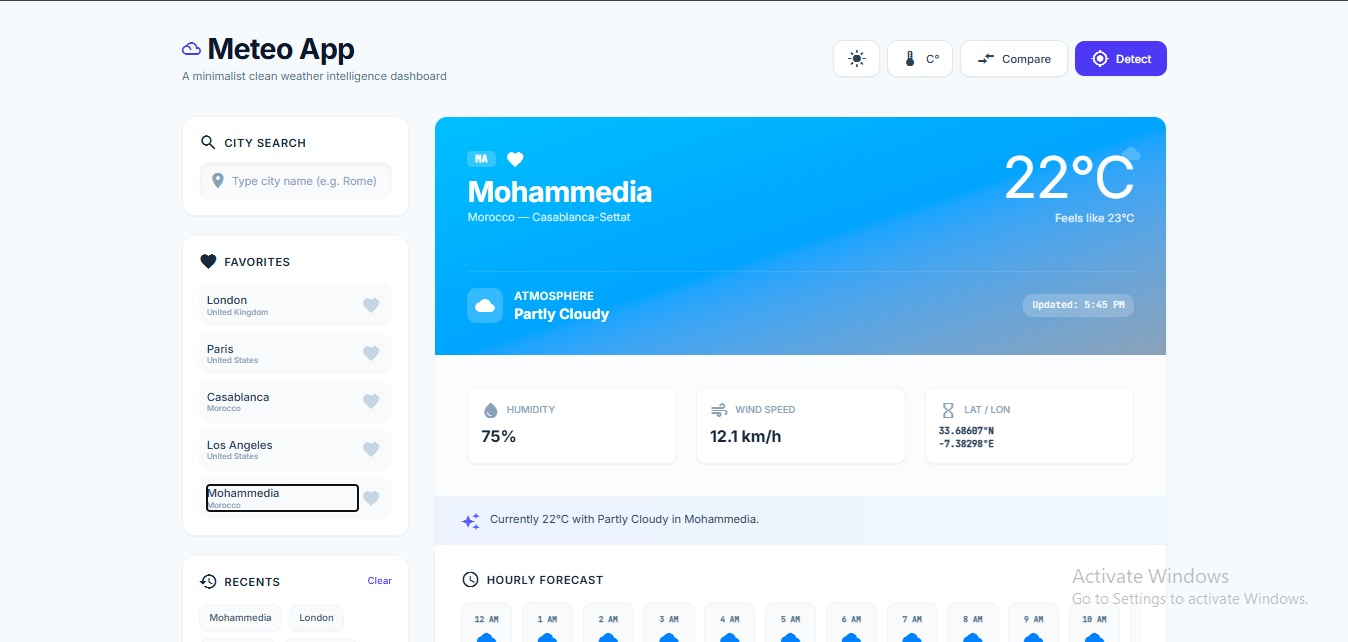
\includegraphics[width=\textwidth,height=0.3\textheight,keepaspectratio]{images/dashboard.jpeg}
\caption{Page d'accueil avec recherche et conditions actuelles}
\label{fig:dashboard}
\end{figure}

La figure~\ref{fig:dashboard-suite} montre la suite de la page d'accueil avec le graphique des températures sur 5~jours et l'indice de qualité de l'air.

\begin{figure}[H]
\centering
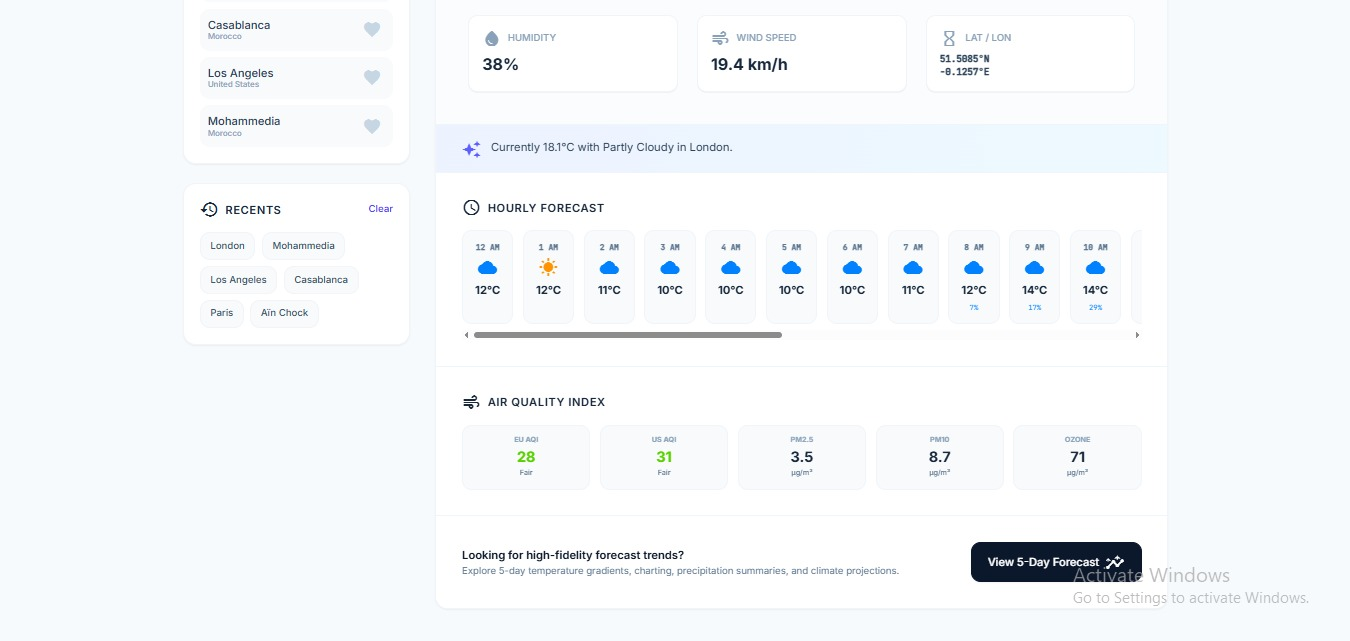
\includegraphics[width=\textwidth,height=0.3\textheight,keepaspectratio]{images/dashboard-suite.jpeg}
\caption{Graphique des températures et qualité de l'air}
\label{fig:dashboard-suite}
\end{figure}

\subsection{Previsions detaillees}

La figure~\ref{fig:forecast} illustre la page de previsions detaillees avec les informations completees (vent, humidité, pression).

\begin{figure}[H]
\centering
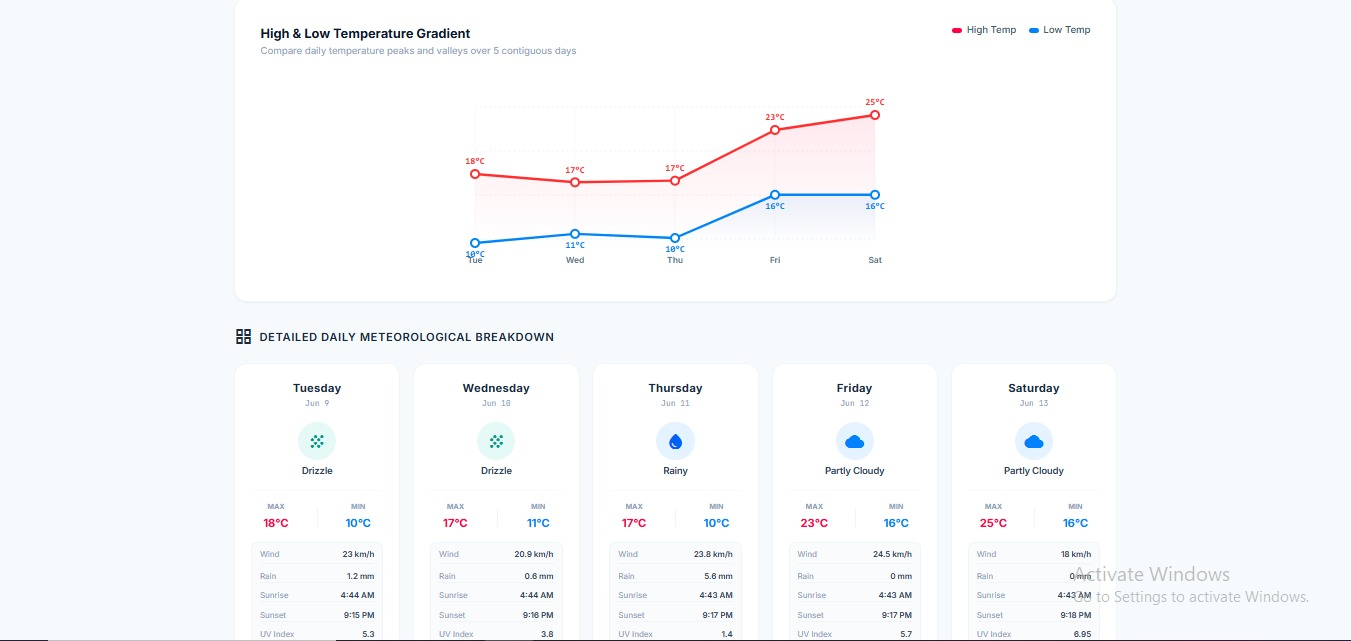
\includegraphics[width=\textwidth,height=0.3\textheight,keepaspectratio]{images/forecast.jpeg}
\caption{Page de previsions detaillees}
\label{fig:forecast}
\end{figure}

\subsection{Comparaison de villes}

Les figures~\ref{fig:comparison} et~\ref{fig:comparison-suite} montrent la fonctionnalité de comparaison entre deux villes avec les cartes jour par jour et les indicateurs cote-a-cote.

\begin{figure}[H]
\centering
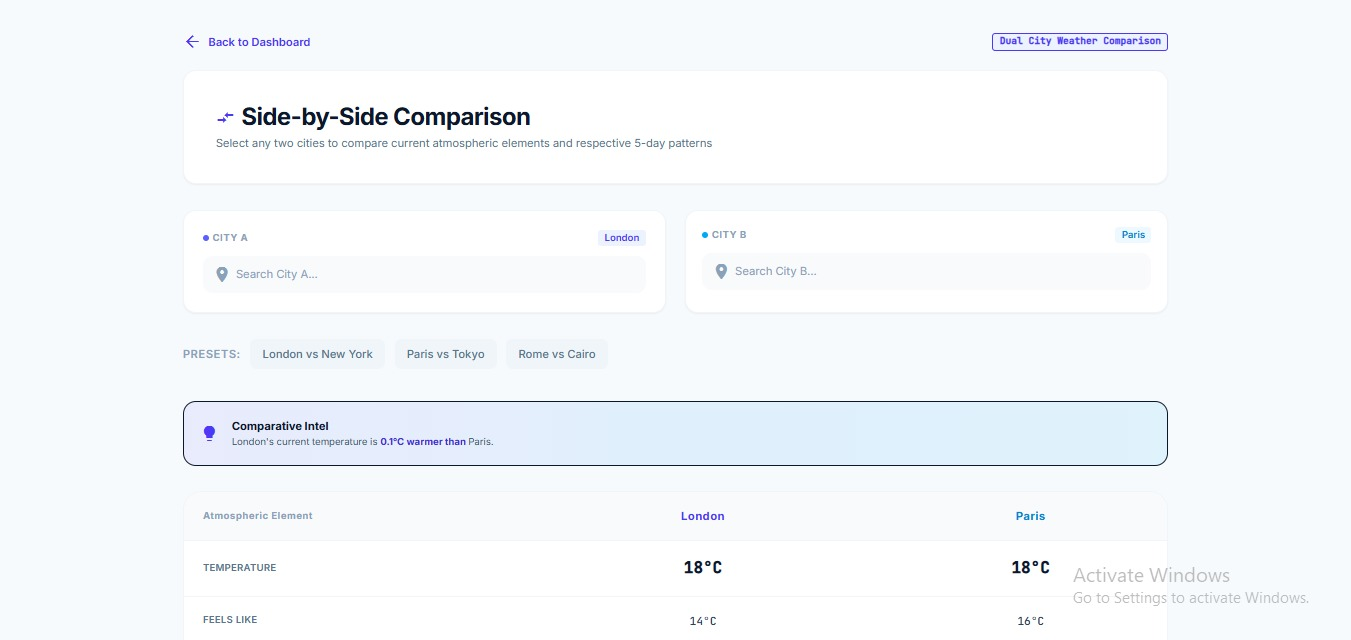
\includegraphics[width=\textwidth,height=0.3\textheight,keepaspectratio]{images/comparison.jpeg}
\caption{Comparaison de deux villes (partie 1)}
\label{fig:comparison}
\end{figure}

\begin{figure}[H]
\centering
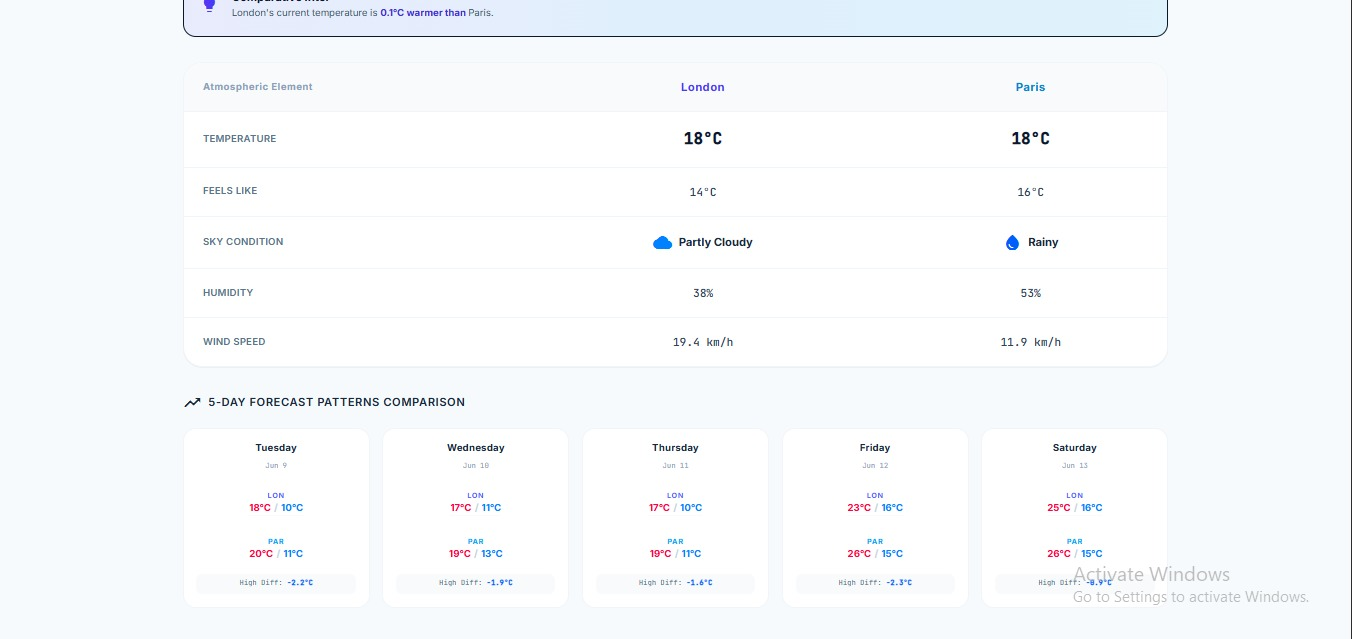
\includegraphics[width=\textwidth,height=0.3\textheight,keepaspectratio]{images/comparison-suite.jpeg}
\caption{Comparaison de deux villes (partie 2)}
\label{fig:comparison-suite}
\end{figure}

% ──────────────────────────────────────────────────────────────────────
\newpage
\section{Conclusion}
\label{sec:concl}

\subsection{Bilan technique}

Ce projet a permis de mettre en œuvre l'ensemble des concepts fondamentaux d'Angular 21 :

\begin{itemize}[nosep]
    \item \textbf{Architecture standalone} : composants, routes et configuration sans \texttt{NgModules}
    \item \textbf{Gestion d'état reactive} : \texttt{signal()}, \texttt{computed()}, detection \texttt{OnPush}
    \item \textbf{Formulaires réactifs} : \texttt{FormControl}, debounce, \texttt{switchMap}
    \item \textbf{HTTP et RxJS} : \texttt{HttpClient}, \texttt{forkJoin}, \texttt{catchError}
    \item \textbf{Routage} : routes paramètrees, \texttt{ActivatedRoute}, navigation
    \item \textbf{SSR} : rendu serveur avec Express, modes Server et Prerender
    \item \textbf{Animations SVG} : calcul de coordonnees, \texttt{stroke-dasharray}, \texttt{requestAnimationFrame}
    \item \textbf{Persistance} : \texttt{localStorage} avec protection SSR
    \item \textbf{Tests} : Vitest, \texttt{HttpTestingController}
    \item \textbf{Intégration API} : trois API REST externes orchestrées
\end{itemize}

\subsection{Défis techniques}

Les principaux défis rencontres incluent :
\begin{itemize}[nosep]
    \item La coordination des appels API parallèles avec \texttt{forkJoin}
    \item L'animation du graphique SVG sans bibliotheque externe
    \item La gestion des états de chargement, d'erreur et de donnees vides (skeleton, erreur, contenu)
    \item La synchronisation des états entre les composants via le service partage
    \item Le rendu SSR avec des paramètres de route dynamiques
\end{itemize}

\subsection{Perspectives}

Plusieurs améliorations pourraient être apportées :
\begin{itemize}[nosep]
    \item Graphiques supplémentaires (précipitations, vent, pression atmosphérique)
    \item Internationalisation (i18n) avec \texttt{@angular/localize}
    \item Progressive Web App (PWA) avec \texttt{@angular/pwa}
    \item Tests de bout en bout avec Cypress ou Playwright
    \item Optimisations avec \texttt{defer} et chargement paresseux (\emph{lazy loading})
\end{itemize}

\end{document}
